\subsection{Sprint 8: da 2024-07-03 a 2024-07-10}
\par In preparazione alla revisione \glossario{RTB}, il team ha fissato come obiettivo principale l’aggiornamento e la revisione della documentazione prodotta fino allo sprint corrente. Per quanto riguarda i singoli documenti, l’attività prioritaria è la stesura finale del cruscotto di valutazione della qualità nel \PdQ. Inoltre presentare il \glossario{PoC} alla Proponente.

\subsubsection{Obiettivi}
\begin{itemize}
  \item Aggiornamento della documentazione in preparazione alla prima fase della revisione \glossario{RTB};
  \item Completamento \glossario{PoC};
  \item Revisione delle metriche di processo e di prodotto;
  \item Suddivisione delle metriche in base all'obiettivo.
\end{itemize}

\begin{figure}[H]
  \centering
  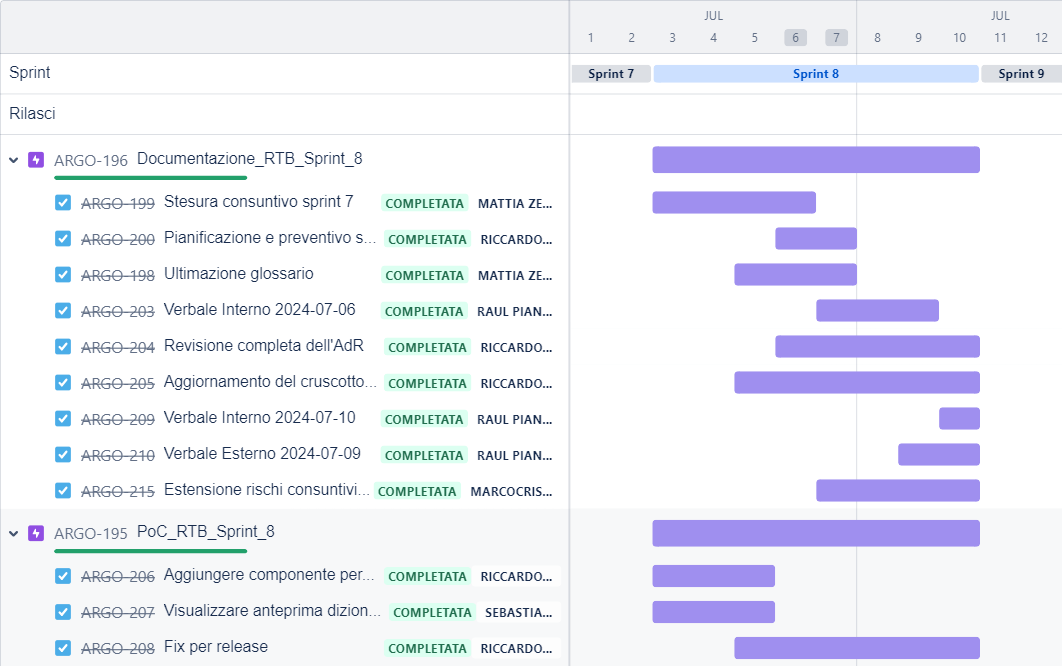
\includegraphics[width=0.90\textwidth]{assets/Pianificazione/Sprint-8/gantt.png}
  \caption{Sprint 8 - Diagramma di Gantt}\label{fig:sprint-8-gantt}
\end{figure}
